\documentclass[12pt]{article}

\usepackage{sbc-template}
\usepackage[brazil,american]{babel}
\usepackage[utf8]{inputenc}

\usepackage{graphicx}
\usepackage{url}
\usepackage{float}
\usepackage{listings}
\usepackage{color}
\usepackage{todonotes}
\usepackage{algorithmic}
\usepackage{algorithm}
\usepackage{hyperref}
\usepackage{indentfirst}
\usepackage{longtable}
\usepackage[inline]{enumitem}


\graphicspath{{./images/}}

\sloppy

\title{Laboratório 5\\- CPU MIPS Pipeline –}

\author{GRUPO 6\\
	Dayanne Fernandes da Cunha, 13/0107191\\
	Lucas Mafra Chagas, 12/0126443\\
	Marcelo Giordano Martins Costa de Oliveira, 12/0037301\\
	Lucas Junior Ribas, 16/0052289\\
	Caio Nunes de Alencar Osório, 16/0115132\\
	Diego Vaz Fernandes, 16/0117925}

\address{Dep. Ciência da Computação -- Universidade de Brasília (UnB)\\
  CiC 116394 - OAC - Turma A
  \email{}
}

\begin{document}
\maketitle

\section{Objetivos}
\label{sec:Objetivos}

\begin{itemize}
\item Treinar o aluno com a linguagem de descrição de \textit{hardware} \textit{Verilog};
\item Familiarizar o aluno com a plataforma de desenvolvimento \textit{FPGA DE2} da \textit{Altera} e o software \textit{QUARTUS II};
\item Desenvolver a capacidade de análise e síntese de sistemas digitais usando uma Linguagem de Descrição de \textit{Hardware};
\item Apresentar ao aluno a implementação de uma \textit{CPU MIPS Pipeline}.
\end{itemize}

\section{Ferramentas}
\label{sec:Materiais}

Todos os códigos escritos neste laboratório podem ser encontrados no repositório \url{https://github.com/Dayof/OAC172} do \textit{GitHub}.

\begin{itemize}
\item FPGA DE2 da Altera 
\item QUARTUS-II
\item Verilog HDL
\end{itemize}

\section{Exercício 2. Análise do processador Pipeline}
\label{sec:pipeline}

\subsection{Diagrama de Blocos do Caminho de Dados}

\begin{figure}[H]
	\flushleft
	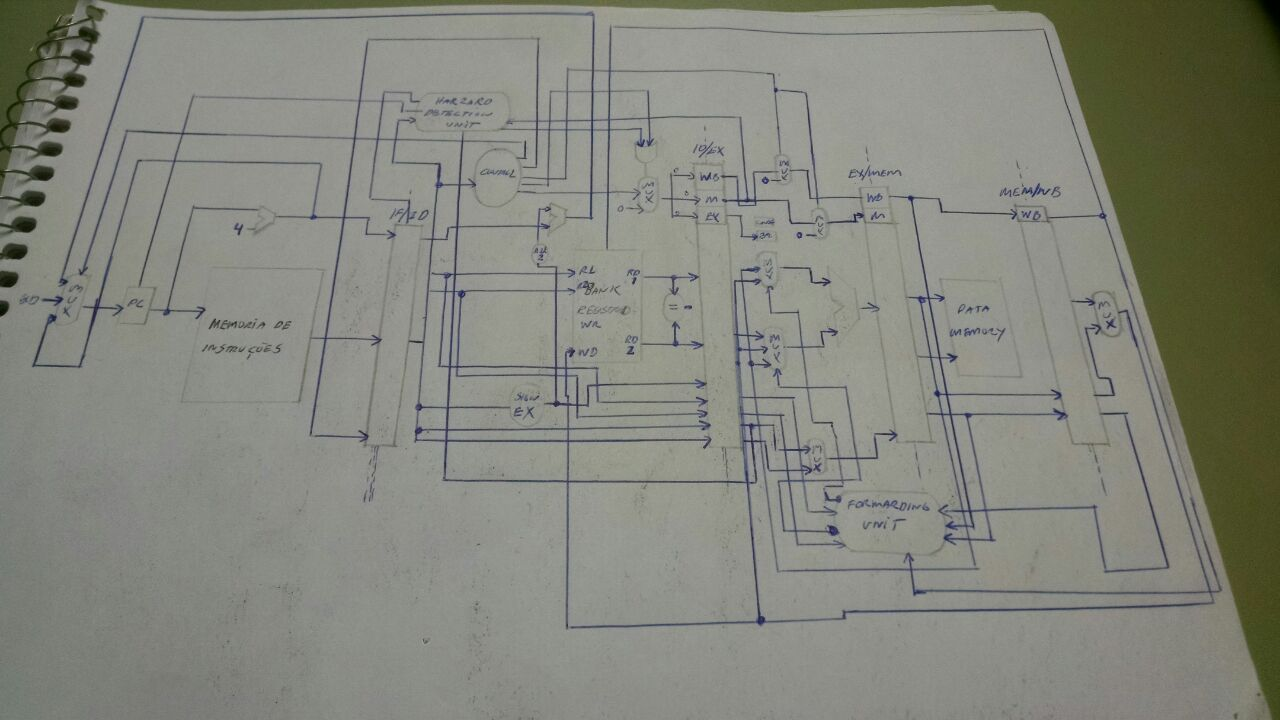
\includegraphics[width=1\textwidth]{caminho_de_dados.jpg}
	\caption{Diagrama de Blocos do Caminho de Dados.}
	\label{fig:pfunct}
\end{figure}

\subsection{Tabela Verdade dos Sinais de Controle}

\section{Exercício 3. Análise unidades de Hazard e Forward}
\label{sec:hazardforward}

A unidade de Fowarding detecta e trata os hazards que podem acontecer com instruções nas etapas EX e WB, mais especificamente em operações que tentam ler registradores que estão sendo modificados por instruções em etapas posteriores do processador.

 add \$t0, \$t1, \$t2 
 add \$t3, \$t0, \$t0 

é um exemplo e

 add \$t0, \$t1, \$t2 
 sub \$s0, \$s1, \$s2 
 add \$s0, \$t0, \$t0 

também.

A unidade de Hazard implementada trata os casos:

-  Desvio condicional (beq, bne), que dão flush na etapa anterior para que aconteça o desvio.

 bne \$t0, \$t1, LABEL
 add \$t0, \$t1, \$t2

- jr, quando uma instrução em EX tiver o registrador destino igual ao Rs da instrução em ID ou a instrução em Mem for escrever em \$ra.

 addi \$ra, \$ra, 0x0AC 
 jr \$ra 

-lw, caso padrão onde alguma instrução precisa do valor que ainda não foi modificado na memória.

lw \$t0, 0 (\$t1)
sub \$t2, \$t1, \$t1


Esses casos foram observados na ISA implementada.

\section{Exercício 4. Teste do funcionamento das instruções da \textit{ISA} }
\label{sec:testeisa}

A demonstração e explicação do código estão presentes nos seguintes vídeos:

\begin{itemize}
\item \href{https://youtu.be/u5eFv9_BDSw}{Formas de Onda}
\item \href{https://youtu.be/PA9af2_Dhi4}{Implementação na DE2} 
\end{itemize}


\section{Exercício 5. Software de lançamento de bola de canhão na \textit{FPGA}}
\label{sec:canhao}

Segue a simulação da bola de canhão:

\href{https://youtu.be/4IZcH5GzhVk}{Bola de canhão}


\section{Exercício 6. Implementação do Cartão SD}
\label{sec:cartaosd}

As limitações observadas ao executar os cenários no cartão sd e impressas no monitor através de um cabo vga foram:

\begin{itemize}
\item 
\item 
\end{itemize} 

Segue o vídeo dos cenários:

\href{https://youtu.be/VeoxltP3L6o}{Cenários no cartão SD}

  
\section{Exercício 7. Novas instruções usando a \textit{ISA MIPS}}
\label{sec:isamips} 

\subsection{Parêmtros}
\label{subsec:param}


\subsection{Caminho de dados}
\label{subsec:datapath}


\subsection{Bloco de controle}
\label{subsec:control}


\subsection{Teste das novas instruções}
\label{subsec:testeisa}


\bibliographystyle{sbc}
\bibliography{relatorio}

\end{document}
